\chapter{Requirement Specifications} \label{chap:reqs}

%\version{v1.10.2015}

\section*{}
\section{Existing System}
The wholesale and bulk trading industry in Pakistan has been traditionally relying on middlemen, personal contacts, and face-to-face communication. There have been a number of digital B2B platforms developed to fill this gap, such as Alibaba, IndiaMart, TradeKey Pakistan and local classifieds like OLX and PakWholesalers. The purpose of these platforms is to match buyers and sellers on a digital platform, yet they cannot meet the needs of the small and medium enterprise (SME) sector of Pakistan specifically \cite{ali2022ecommerce}. The majority of these platforms are either too generic to conduct local business or offer functionalities that are too few to facilitate efficient bulk trade and direct business negotiations \cite{hussain2023supply}.

\subsection{Limitations of the Existing System}
The already existing B2B platforms, though useful in a number of ways, have grave shortcomings in terms of catering to the unique needs of Pakistani manufacturers, wholesalers, and retailers:

\begin{itemize}
    \item The absence of real-time communication between buyers and sellers and, therefore, slow and inefficient negotiations.
    \item Lack of multilingual assistance (especially Urdu), restricting access to local businesses \cite{akram2022user}.
    \item Lack of an built-in Request for Quotation (RFQ) system to negotiate custom bulk-orders.
    \item No tiered or bulk pricing models to support wholesale transactions.
    \item  Interfaces that are complicated enough to be inaccessible to small sellers or too simple to allow growing businesses to develop further \cite{han2023digital}.
    \item Lack of mobile optimization and thus poor user experiences on smartphones.
    \item No AI assisted product review analysis or market knowledge.
    \item Absence of push notification systems to give prompt order and communication notices.
    \item Overdependence on intermediaries, rising costs, decreasing transparency of the supply chain \cite{raza2023impact}.
\end{itemize}

\section{Proposed System}
Indus Bazar is a mobile based B2B marketplace application, which aims to directly integrate manufacturers, wholesalers, and retailers in a single digital platform. The system offers an all-inclusive collection of applications that allows business to find products, negotiate bulk purchases, make transactions, and communicate in real time, all in one application \cite{farooq2024mobile}. The platform was developed with Flutter, Dart, and Appwrite, supporting both Urdu and English, which will provide the appropriate cultural alignment and allow Pakistani users to use it. Indus Bazar combines artificial intelligence-driven review summarization, secure Stripe payment processing, a Request for Quotation (RFQ) marketplace, tiered bulk pricing, and chat to provide a seamless, transparent and efficient B2B commerce experience.

\subsection{The Proposed System Overcomes the Limitations of the Existing Systems.}
the Limitations of the Existing Systems.
To directly overcome the limitations of the current systems, the following innovative features are applied by Indus Bazar:

\begin{itemize}
    \item Will offer a live chat platform that will allow buyers and sellers to communicate instantly and negotiate directly.
    \item Provides support of Urdu and English interface to provide accessibility and cultural suitability to Pakistani users \cite{akram2022user}.
    \item It has an exclusive RFQ (Request for Quotation) Marketplace, where a customer can post requests on items, and sellers compete to offer the best price.
    \item Adopts the levels of pricing to facilitate bulk buying with automatic price discounts according to the order quantity.
    \item Provides a mobile-first, easy to use, user-friendly interface that works well with Android devices and is scalable to businesses of any size \cite{farooq2024mobile}.
    \item Incorporates AI-enhanced review summarization to enable buyers to make a wise choice and aid sellers in gaining insight into customer feedbacks \cite{chaffey2022digital}.
    \item Supports push notifications to deliver timely order, chat, and system updates.
    \item Minimizes the need to intermediaries by allowing direct digital links between both manufacturers and buyers, decreasing expenses and enhancing transparency \cite{hussain2023supply}.
\end{itemize}

\section{Requirements Specifications}
System requirements are divided into functional and non-functional requirements for an optimum and user-friendly platform. Functional requirements refer to the set of features and functionalities that the system should possess in order to address the needs of customers and sellers in the Indus Bazar marketplace. Non-functional requirements focus on system quality, security and performance issues to address the needs of system usability.  The functional and non-functional requirements are necessary to develop the Indus Bazar as a secure, scalable and accessible B2B marketplace for Pakistan‘s digital economy.

\section{Functional Requirements}
Functional requirements: define the essential functions provided by the Indus Bazar platform to enable complete B2B commerce functionality. These requirements dictate the expected system behaviour for the customer-side functionality (such as login,  browse and select products,  place purchase orders,  and payment) and seller-side functionality (such as login,  add/edit/remove products,  and balance invoice requests); and include the RFQ marketplace,  turn-based communication, and notification services.  Every functional requirement can be traceably linked to use cases that have been identified during the analysis phase,  and can be linked to a testable functionality that must be developed prior to deployment.

\subsection{Login and Registration}
\begin{itemize}
    \item Customers and sellers can register their name, email address, and secure password in the system using a registration form and choose their role (Customer or Seller).
    
    \item When a user registers, a verification email is sent to the provided email address. The user is allowed to access the system only after verifying the email by clicking a deep link.
    
    \item Registered users can log into the system using their email and password. Upon successful authentication, role-based access is provided to either the customer or seller dashboard.
    
    \item The system includes a password recovery option that uses the registered email, allowing users to reset their credentials securely.
    
    \item Role-Based Access Control (RBAC) is implemented to ensure that customers and sellers can only access functions and information relevant to their roles.
\end{itemize}

\subsection{Product Catalog Management}
\begin{itemize}
    \item The system offers a tabular product listing with categories and subcategories, including product descriptions, specifications, and prices.
    
    \item The search engine allows users to find products using keywords, filters (category, price range, and seller), and sorting options to efficiently identify the desired products.
    
    \item Tiered pricing information is displayed in each product listing, with clear per-unit pricing at various order quantity levels.
    
    \item Sellers can add, edit, and delete items in their listings via the seller dashboard, and updates are immediately reflected in the catalog.
    
    \item The system supports multilingual product names and descriptions in both English and Urdu to enhance accessibility.
\end{itemize}

\subsection{Shopping Cart and Checkout}
\begin{itemize}
    \item Shoppers can add or remove items from the shopping cart and modify item quantities before proceeding to checkout.
    
    \item The system automatically calculates the tiered price based on the selected quantity of each product.
    
    \item During checkout, customers can select an existing delivery address or add a new one and confirm the final order summary.
    
    \item The checkout process is streamlined and validated to prevent incomplete or incorrect order submissions.
    
    \item Customers can manage multiple delivery addresses and assign a default address for faster checkout.
\end{itemize}

\subsection{Secure Payment Integration}
\begin{itemize}
    \item The system has been built to connect with Stripe as the payment gateway to enable safe online payments. It is still in test as to confirm the payment workflow.
    
    \item The server-side Appwrite functions are used to process payment to make sure that payment information is never sent to the client-side in an exposed form.
    
    \item It will accept card payments and give real-time payment confirmation or failure messages.
    
    \item The order is automatically created and a push notification sent to the seller associated with the order when it is successfully paid.
    
    \item The records of transactions are well-protected and are accessible to clients and merchants via order histories.
\end{itemize}

\subsection{Order Management}
\begin{itemize}
    \item The system handles all order lifecycle, such as order placement, order processing, order dispatch, and order delivery.
    
    \item Customers are able to use their order history dashboard to track the status of their orders.
    
    \item sellers have access to incoming orders, update on order statuses (Confirmed, Processing, Shipped, Delivered or Cancelled) and fulfillment through the seller dashboard.
    
    \item When an order status is updated, customers and sellers get a push notification.
    
    \item The system has a detailed history of order to aid in business record-keeping and resolving disputes.
\end{itemize}

\subsubsection{Tiered Pricing and Bulk Ordering}
The system also has a tiered pricing model to promote bulk buying. The unit cost reduces with the quantity of order, thus appealing to the retailers and wholesalers to purchase in large quantities. The following table is an example of a tiered pricing structure:

\renewcommand{\arraystretch}{1.2}
\begin{longtable}{|l|l|l|}
\caption{Tiered Pricing Structure Example}\label{tab:tiered_pricing}\\
\hline
\rowcolor{lightgray}
\textbf{Tier} & \textbf{Minimum Order Quantity} & \textbf{Price Per Unit}\\
\hline
\endhead
Tier 1 (Base) & 1+ units & PKR 1,000 per unit\\
\hline
Tier 2 (Wholesale) & 50+ units & PKR 850 per unit\\
\hline
Tier 3 (Bulk) & 100+ units & PKR 700 per unit\\
\hline
\end{longtable}
\renewcommand{\arraystretch}{1}


The tiered pricing model allows sellers to establish a fixed price level of a product, up to three, each having a limited order quantity and a unit price. The price tier to be applied is automatically calculated by the system depending on the amount of units the customer chooses, the higher the units the cheaper the unit price.

The product detail page shows all the pricing levels. Before adding products to their cart, customers have the chance to change the quantity to take advantage of discounted prices. In case of a large order or a tailored order, customers are welcome to negotiate the price directly with the sellers using the RFQ Marketplace.

\subsection{Real-Time Chat System}
\begin{itemize}
    \item The system has a real-time chat option that allows direct customer-seller communication.
    
    \item Text and image messaging is enabled and sellers can share product photos, catalogues, and documents with buyers.
    
    \item Conversations are user specific, and are continuously archived, allowing users to re-examine previous conversations.
    
    \item Push messages inform users immediately about new messages, which helps to respond quickly and negotiate faster.
    
    \item There is chat functionality on both product listing and order page where it can easily be used to communicate.
\end{itemize}

\subsection{RFQ (Request for Quotation) Marketplace}
\begin{itemize}
    \item The system has a dedicated RFQ Marketplace where customers can make requests concerning the items they need such as product name, category, quantity, delivery city, delivery date, optional price range (minimum and maximum) and other specifications.
    
    \item RFQ listings are open to seller quotes of a period up to seven days, and will automatically expire unless a quote is accepted.
    
    \item Sellers are able to see active RFQs and place competitive bids with unit price and total price, expected time of delivery and notes.
    
    \item Push messages are delivered to the customers every time a new quote is offered, and the customers can review, compare and accept the most appropriate offer.
    
    \item Accepted quotations are automatically turned into order to be checked out with the agreed price applied, and competing quotations are rejected.
    
    \item RFQ option will remove the necessity of any external communication channels and provide clear, well-documented trade negotiations inside the platform.
\end{itemize}

\subsection{AI-Powered Review Summarization}
\begin{itemize}
    \item The system has an AI-powered module which analyzes reviews of customers of specific products and creates readable short summary on-demand.
    
    \item Summaries are initiated by the user. On clicking the \textit{Generate Summary} button on the product detail page, an Appwrite cloud functions produces the summary in the chosen language.
    
    \item Summaries come in both Urdu and English. The product detail page has a toggle option which enables the user to use alternative languages without re-generating the summary.
    
    \item Reviews are only allowed to people who have made confirmed purchases of the product i.e. people who have placed non-refunded orders and the product received.
    
    \item AI-generated summaries enable sellers to swiftly comprehend customer sentiment in general, and areas of product or service enhancement.
    
    \item The AI part of the platform can only review summarization in the current version.
\end{itemize}

\subsection{Push Notifications}
\begin{itemize}
    \item The system provides real-time push notifications of crucial events like order placements, status updates, chat messages, and RFQ related events.
    
    \item Firebase Cloud Messaging (FCM) and Appwrite messaging services are used to implement the notifications.
    
    \item Customers and sellers get role specific notifications to keep them posted on their activities on the platform.
    
    \item The app has an option of viewing the history of notification in the future.
    
    \item The notification system works when the application is not in the background or after closing the application.
\end{itemize}

\subsection{Report Generation}
\begin{itemize}
    \item Order History: The users can get a full view of their order history including the order dates, products, quantities, totals and the statuses.
    
    \item Transaction Records: Views all financial transactions by customers or to sellers, including Stripe transaction IDs and times.
    
    \item Seller Sales Overview: Sellers will have access to aggregate sale information, such as fulfilled orders, total revenue, and products sold most.
    
    \item RFQ Activity: Tracks the submitted quotes, accepted deals, pending negotiations by the sellers and the submitted requests by the customers.
    
    \item{Review Analytics: The product performance of the sellers can be tracked using AI-generated summaries of reviews and customer feedback in a single dashboard.
\end{itemize}

\subsection{Administrative Functions}
\begin{itemize}
    \item Seller Dashboard: Sellers can use a special dashboard where they can see an overview of active posts, orders, active chat, and quotes.
    \item Product Management: Sellers are able to add and update their listings, control pricing levels, and delete discontinued products.
    \item Order Fulfillment Control: Sellers can change the status of orders at all points throughout the fulfillment lifecycle and attach tracking or delivery notes.
    \item Quote Management: Sellers are able to handle all quoted items, monitor accepted and pending RFQ requests, and respond to customer requests.
    \item Performance Monitoring: AI-generated summary of reviews and order statistics can help sellers track product performance and customer feedback to optimize their offerings.
\end{itemize}

\section{Non-Functional Requirements}
\begin{itemize}
    \item \textbf{Security:} The system should be equipped with strong authentication, role-based access control, email authentication, and secure server-side payment processing to secure user accounts and sensitive business data.
    
    \item \textbf{Performance:} The site should be able to provide quick load times, chat responsiveness in real time, and timely push notifications to have an efficient user experience on all core functionality.
    
    \item Scalability The system should have the ability to handle an increasing number of simultaneous users, product entries, and transactions without affecting its performance negatively (Laudon 2023ecommerce).
    
    \item Availability: The platform should be highly available to guarantee that users can access the marketplace, manage orders and communicate any time.
    
    \item \textbf{Usability:} The interface needs to be simple and user-friendly to both small and large business with a mobile-first design that is Android-friendly.
    
    \item Multilingual Support: The system should be bilingual in Urdu and English, covering both main interface elements and the content of the products and AI-generated summaries to address the needs of the diverse Pakistani market.
    
    \item Data Privacy and Compliance: The system should guarantee the privacy of user data, business data and transaction records by deploying proper encryption and access control.
\end{itemize}

\section{User Requirements}
\begin{itemize}
    \item \textbf{Customer Registration and Login.}
    \begin{itemize}
        \item The ability to create an account including name, email, password, and role choice (Customer or Seller).
        \item Before accessing the platform email validation is to be done.
        \item protected log-in and access to a role-based, personalized dashboard.
        \item Recovery of passwords through registered email.
    \end{itemize}

    \item \textbf{Product Discovery}
    \begin{itemize}
        \item The ability to navigate a structured product catalog in categories and subcategories.
        \item Advanced search and filtering features in order to find certain products fast.
        \item Tiered pricing information on the product detail page.
        \item Read AI-generated review summaries in English or Urdu to make an informed purchase.
    \end{itemize}

    \item \textbf{Shopping Cart and Checkout.}
    \begin{itemize}
        \item Add products to a cart, change quantities, and preview prior to checking out.
        \item Add more than one address to be used when making a delivery.
        \item Simplified checkout experience and automatic calculation of price tiers.
    \end{itemize}

    \item \textbf{Payment and Order Management.}
    \begin{itemize}
        \item Card-based payment processing using Stripe with real-time confirmation.
        \item Full order history with tracking of status, starting with placement through delivery.
        \item Push notifications of all changes of order status.
    \end{itemize}

    \item \textbf{RFQ and Negotiation.}
    \begin{itemize}
        \item Capacity to post RFQ requests including product requirements and specifications.
        \item Review and compare quotes posted by several sellers.
        \item Accept desired quote and go straight to checkout at agreed price.
    \end{itemize}

    \item \textbf{Real-Time Communication}
    \begin{itemize}
        \item Face to face negotiation, communication, and clarification with the sellers.
        \item Text and image message support in chat interface.
        \item Real time push notifications of new messages.
    \end{itemize}

    \item \textbf{Seller Registration and Dashboard.}
    \begin{itemize}
        \item Sellers will have the opportunity to register, verify their email and get a dedicated seller dashboard.
        \item Product listing product listing and product listing additions/updates/removals with tiered pricing.
        \item See and complete incoming customer orders with status update features.
        \item Respond to RFQ requests by customers.
        \item observe the performance of products with a review summary and sales report.
    \end{itemize}

    \item \textbf{Multilingual Accessibility}
    \begin{itemize}
        \item Platform interface and AI-generated summaries (both English and Urdu).
        \item Simple, interactive design that can be used by various users in Pakistan.
    \end{itemize}

    \item \textbf{Availability}
    \begin{itemize}
        \item Platform available 24/7 to facilitate business operations and time sensitive transactions.
    \end{itemize}
\end{itemize}

\section{Use Case Diagram}

In this section, the UML Use Case Diagrams of the Indus Bazar B2B Marketplace Application will be provided and the key interactions between the system and the two main actors, the Customer and the Seller in the core functional areas of the system.

\subsection{Customer System Use Case}
The Customer System Use Case diagram below shows the entire list of interactions that a customer is able to achieve on the Indus Bazar platform, such as authentication, product-finding, purchasing, and bargaining processes.

\begin{figure}[H]
\centering
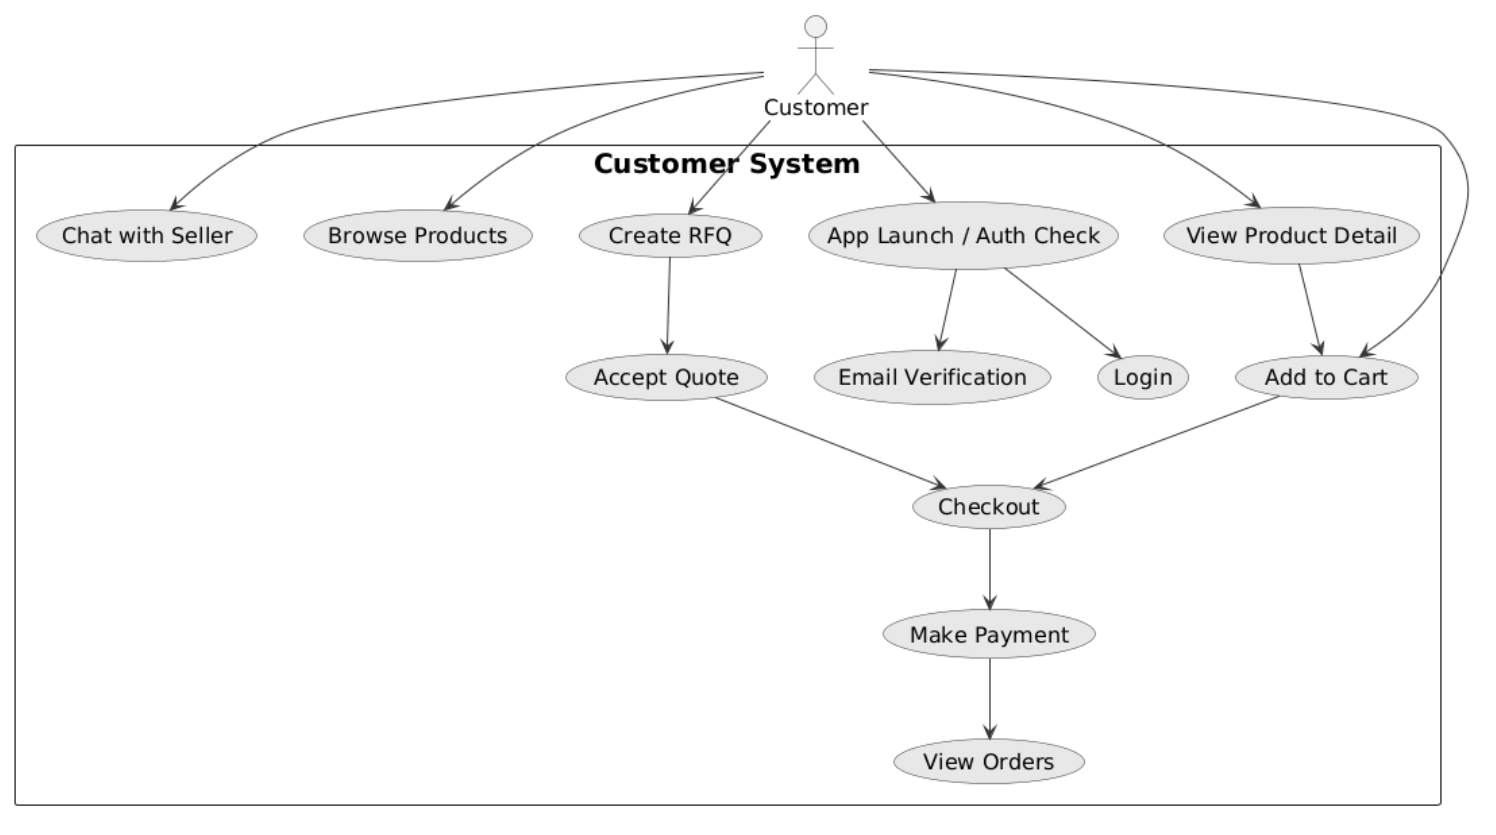
\includegraphics[width=0.95\textwidth]{figures/pictures project/customer_usecase.png}
\caption{Customer System Use Case Diagram}
\label{fig:customer_use_case_diagram}
\end{figure}

The use case diagram shown in Figure \ref{fig:customer_use_case_diagram} demonstrates all the possible interactions that the Customer actor can have in the Indus Bazar system. The diagram illustrates:

\begin{itemize}
    \item \textbf{Primary Actor:} Customer communicating with all core purchasing and communication functions.

    \item \textbf{Authentication Flow:}
    \begin{itemize}
        \item App Launch / Auth Check - system checks whether the user has already been authenticated on launch.
        \item Login - Customer enters the credentials to enter the platform.
        \item Email Verification - after initial registration, they need to go through the email verification.
    \end{itemize}

    \item \textbf{Core Use Cases:}
    \begin{itemize}
        \item Browse Products — customer browses products catalog.
        \item View Product Detail Customer sees detailed product information and tiered pricing.
        \item Develop RFQ customer makes a request of quotation of bulk or custom orders.
        \item Chat with Seller — customer is in direct communication with a seller.
        \item Accept Quote - customer reviews the quote that has been submitted by a seller and accepts it.
        \item Add to Cart — customer will add items to the shopping cart.
        \item Checkout Customer reviews cart and selects address to deliver to and confirms order.
        \item Make Payment - customer makes the payment using Stripe.
        \item View Orders — customer follows orders placed and order history.
    \end{itemize}
\end{itemize}

\subsection{Seller System Use Case}

The Seller System Use Case diagram below displays the interaction that can be offered to a seller on the Indus Bazar platform and includes the activities of authentication, product management, order fulfillment, and interaction with customers.

\begin{figure}[H]
\centering
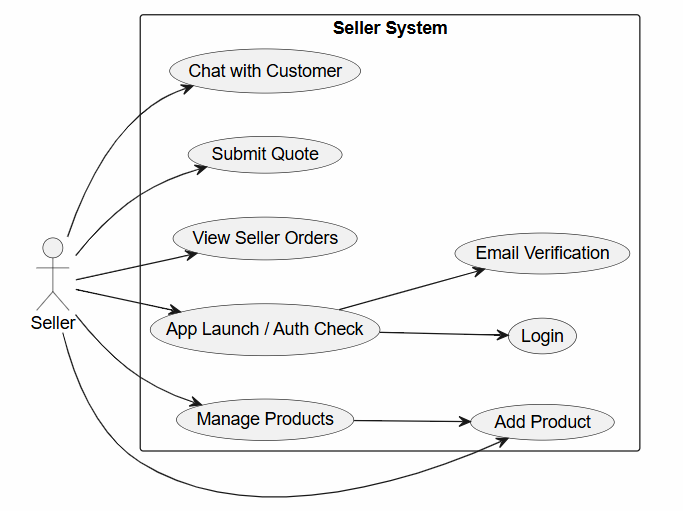
\includegraphics[width=0.85\textwidth]{figures/pictures project/seller_usecase.png}
\caption{Seller System Use Case Diagram}
\label{fig:seller_use_case_diagram}
\end{figure}

The use case diagram shown in Figure \ref{fig:seller_use_case_diagram} illustrates the seller-side interactions within the Indus Bazar system. The diagram illustrates:

\begin{itemize}
    \item \textbf{Primary Actor:} Seller managing products, orders, quotes, and customer communication.

    \item \textbf{Authentication Flow:}
    \begin{itemize}
        \item App Launch / Auth Check — system verifies seller session status on launch
        \item Login — seller authenticates to access the seller dashboard
        \item Email Verification — mandatory on registration for seller account activation
    \end{itemize}

    \item \textbf{Core Use Cases:}
    \begin{itemize}
        \item Manage Products — seller manages the full lifecycle of product listings
        \item Add Product — seller creates new product listings with pricing tiers and details
        \item Submit Quote — seller responds to customer RFQ requests with competitive offers
        \item View Seller Orders — seller monitors and fulfills incoming customer orders
    \end{itemize}
\end{itemize}

\subsection{Use Case Specifications}

This section gives the important specifications of each of the use cases in the Indus Bazar system, including use case ID, name, actors, preconditions, basic flow, alternative flows, and postconditions, in a tabular form.

\subsubsection{Login}
The use case of login, as illustrated in the table below (Login) \ref{tab:use_case_login} outlines how the registered customers and sellers can securely access the Indus Bazar platform and its services. 
\renewcommand{\arraystretch}{1.3}
\begin{longtable}{|p{3cm}|p{10cm}|}
\caption{Use Case - Login}\label{tab:use_case_login}\\
\hline
\rowcolor{lightgray}
\textbf{Attribute} & \textbf{Description}\\
\hline
\endhead
\textbf{Use Case ID} & UC-01\\
\hline
\textbf{Use Case Name} & Login\\
\hline
\textbf{Actors} & Customer, Seller\\
\hline
\textbf{Description} & Enables registered users to log in securely and access their respective role-based dashboards.\\
\hline
\textbf{Preconditions} & User has a registered and email-verified account.\\
\hline
\textbf{Basic Flow} & 1. User opens the login page.\newline 2. Enters registered email and password.\newline 3. System verifies credentials and determines role.\newline 4. User is redirected to the customer or seller dashboard.\\
\hline
\textbf{Alternative Flows} & Invalid credentials \textrightarrow\ Error message displayed; access denied.\\
\hline
\textbf{Post Conditions} & User is authenticated and directed to the appropriate role-based dashboard.\\
\hline
\textbf{Frequency of Use} & Very Frequent\\
\hline
\textbf{Priority} & High\\
\hline
\end{longtable}

\subsubsection{Registration}
The Registration use case \ref{tab:use_case_registration} enables new customers and sellers to open a new account at the Indus Bazar platform. The system verifies the information given and sends an email verification link through deep link and only after the verification is successful is an access granted. The registration time defines the selection of roles, i.e. the user or seller management dashboard.

\renewcommand{\arraystretch}{1.3}
\begin{longtable}{|p{3cm}|p{10cm}|}
\caption{Use Case - Registration}\label{tab:use_case_registration}\\
\hline
\rowcolor{lightgray}
\textbf{Attribute} & \textbf{Description}\\
\hline
\endhead
\textbf{Use Case ID} & UC-02\\
\hline
\textbf{Use Case Name} & Registration\\
\hline
\textbf{Actors} & Customer, Seller\\
\hline
\textbf{Preconditions} & User does not already have a registered account.\\
\hline
\textbf{Basic Flow} & 1. User opens the registration page.\newline 2. Enters name, email, password, confirm password, and selects role (Customer or Seller).\newline 3. System validates input and creates the account.\newline 4. Verification email is sent to the provided address via deep link.\newline 5. User clicks the verification link and is redirected to login.\\
\hline
\textbf{Alternative Flows} & Email already registered \textrightarrow\ Error message shown.\newline Invalid input format \textrightarrow\ Validation error displayed.\\
\hline
\textbf{Post Conditions} & Account created and email verified; user can now log in.\\
\hline
\textbf{Frequency of Use} & Moderate (once per user)\\
\hline
\textbf{Priority} & High\\
\hline
\end{longtable}

\subsubsection{Browse Products}
The Browse Products use case \ref{tab:use_case_browse_products} enables customer to browse the product offerings of the platform with ease through structured navigation and search features. Users can categorize products, sub categorize them and use the relevant attributes to filter or use key word searches to identify certain products. These inputs are processed by the system and the results that match are retrieved in real time and in a structured and easy to use format. All product listings contain fundamental product data like product name, thumbnail image, seller name and price, which allows a rapid comparison of a variety of products. The system can also be used to facilitate more sophisticated filters like price range, rating or availability to narrow down search results. Where no similar products are located, the system will give useful suggestions or reminders to adjust the search parameters. The use case is crucial in improving product discoverability and overall user experience through making informed decisions.

\renewcommand{\arraystretch}{1.3}
\begin{longtable}{|p{3cm}|p{10cm}|}
\caption{Use Case - Browse Products}\label{tab:use_case_browse_products}\\
\hline
\rowcolor{lightgray}
\textbf{Attribute} & \textbf{Description}\\
\hline
\endhead
\textbf{Use Case ID} & UC-03\\
\hline
\textbf{Use Case Name} & Browse Products\\
\hline
\textbf{Actors} & Customer\\
\hline
\textbf{Description} & Allows customers to search and filter the product catalog to find products meeting their requirements.\\
\hline
\textbf{Preconditions} & Customer is logged in.\\
\hline
\textbf{Basic Flow} & 1. Customer opens the product catalog.\newline 2. Applies category filters or enters search keywords.\newline 3. System displays matching products with thumbnail, price, and seller information.\\
\hline
\textbf{Alternative Flows} & No results found \textrightarrow\ System displays a message suggesting alternative search terms.\\
\hline
\textbf{Post Conditions} & Customer views a filtered list of products matching the search criteria.\\
\hline
\textbf{Frequency of Use} & Very Frequent\\
\hline
\textbf{Priority} & High\\
\hline
\end{longtable}

\subsubsection{View Product Detail}
The View Product Detail use case \ref{tab:use_case_view_product} gives customers a detailed description of a given product, various pictures, a detailed description, stock level, tiered prices, and AI-based customer review summaries. This rich view helps in making an informed bulk buying decision by providing customers with all they require to make an assessment of a product before it is added to the cart or an RFQ is raised. It also emphasizes on major specifications, seller details, and delivery choices to increase transparency. Also, related products and suggestions can be displayed to assist users in searching options and make superior buying decisions.
Product ratings, FAQs, warranty or return policies may also be incorporated into the interface to resolve many issues before they arise. The users can ensure they compare similar products, check bulk rates and estimated delivery dates to plan better. Moreover, the fast features, like adding to wishlist, sharing the product, or contacting the seller directly, enhance user interaction and simplify the decision-making process.


\renewcommand{\arraystretch}{1.3}
\begin{longtable}{|p{3cm}|p{10cm}|}
\caption{Use Case - View Product Detail}\label{tab:use_case_view_product}\\
\hline
\rowcolor{lightgray}
\textbf{Attribute} & \textbf{Description}\\
\hline
\endhead
\textbf{Use Case ID} & UC-04\\
\hline
\textbf{Use Case Name} & View Product Detail\\
\hline
\textbf{Actors} & Customer\\
\hline
\textbf{Description} & Displays full product information including images, specifications, tiered pricing, and AI-generated review summaries.\\
\hline
\textbf{Preconditions} & Customer is logged in; product is listed and active.\\
\hline
\textbf{Basic Flow} & 1. Customer selects a product from the catalog.\newline 2. System displays full product details with all pricing tiers.\newline 3. Customer reviews AI-generated feedback summary and individual reviews.\\
\hline
\textbf{Alternative Flows} & Product unavailable \textrightarrow\ System displays unavailability notice.\\
\hline
\textbf{Post Conditions} & Customer has full visibility of product information and pricing to proceed with cart or RFQ.\\
\hline
\textbf{Frequency of Use} & Frequent\\
\hline
\textbf{Priority} & High\\
\hline
\end{longtable}

\subsubsection{Add to Cart}
The Add to Cart use case \ref{tab:use_case_add_to_cart} enables the customers to choose the products and quantities they want and the system will automatically apply the relevant tiered price depending on the quantity that is entered. This smooth pricing system means that the customers are always shown the right bulk discount automatically without doing any computations and therefore minimizes the chances of error as well as enhances the buying process prior to the checkout counter. The system also checks stock availability within a given time to avoid making an excess order and provides users with any quantity limit or restriction. The quantities of products can be updated, items can be removed or subtotals can be reviewed easily, within the cart. Further, the cart can present an estimate of shipping charges, taxes, and overall prices to offer complete price transparency. Such fast activities as storing goods to be purchased later or visiting a checkout also simplify the process of buying. Persistence may also be supported across sessions by the cart, so that users can resume their shopping at a later time and not lose items picked. Price notifications can be made to notify the users of price changes or stock changes. Moreover, combining with promotions, coupons or special deals will ensure that customers will not miss out any discounts available before making their purchase.

\renewcommand{\arraystretch}{1.3}
\begin{longtable}{|p{3cm}|p{10cm}|}
\caption{Use Case - Add to Cart}\label{tab:use_case_add_to_cart}\\
\hline
\rowcolor{lightgray}
\textbf{Attribute} & \textbf{Description}\\
\hline
\endhead
\textbf{Use Case ID} & UC-05\\
\hline
\textbf{Use Case Name} & Add to Cart\\
\hline
\textbf{Actors} & Customer\\
\hline
\textbf{Description} & Allows customers to add products to the shopping cart with quantity selection and automated tier pricing.\\
\hline
\textbf{Preconditions} & Customer is logged in; product is available.\\
\hline
\textbf{Basic Flow} & 1. Customer selects quantity on product detail page.\newline 2. System applies appropriate tiered price.\newline 3. Customer taps Add to Cart.\newline 4. Item is added to cart with updated totals.\\
\hline
\textbf{Alternative Flows} & Quantity below minimum order threshold \textrightarrow\ System notifies customer of minimum.\\
\hline
\textbf{Post Conditions} & Product is added to the cart with correct tiered pricing applied.\\
\hline
\textbf{Frequency of Use} & Frequent\\
\hline
\textbf{Priority} & High\\
\hline
\end{longtable}

\subsubsection{Checkout}
The Checkout use case \ref{tab:use_case_checkout} is the last step in the purchasing process, during which customers will check and verify their purchase order and move on to payment. The system makes sure that the user must have met all the requirements, such as the cart is not empty and has a valid delivery address before proceeding. It provides a detailed summary of orders which consists of chosen items, quantities, prices, taxes and any other fees to guarantee transparency. This allows customers to have a degree of flexibility and convenience by selecting an existing delivery address or creating a new address. The system carries out end-of-life checks like checking stock level and prices to avoid discrepancies. Error handling systems help users to correct missing or erroneous information. This use case will guarantee that the details of orders are precise and complete before switching to the payment phase and hence reduce the likelihood of a breakdown in these transactions and enhance reliability.
\renewcommand{\arraystretch}{1.3}
\begin{longtable}{|p{3cm}|p{10cm}|}
\caption{Use Case - Checkout}\label{tab:use_case_checkout}\\
\hline
\rowcolor{lightgray}
\textbf{Attribute} & \textbf{Description}\\
\hline
\endhead
\textbf{Use Case ID} & UC-06\\
\hline
\textbf{Use Case Name} & Checkout\\
\hline
\textbf{Actors} & Customer\\
\hline
\textbf{Description} & Guides the customer through order review, address selection, and payment initiation.\\
\hline
\textbf{Preconditions} & Customer is logged in with at least one item in the cart and a delivery address saved.\\
\hline
\textbf{Basic Flow} & 1. Customer opens cart and proceeds to checkout.\newline 2. Reviews order summary and selects delivery address.\newline 3. Confirms order and is directed to payment.\\
\hline
\textbf{Alternative Flows} & No address saved \textrightarrow\ Customer is prompted to add a delivery address.\\
\hline
\textbf{Post Conditions} & Order details confirmed; customer proceeds to payment.\\
\hline
\textbf{Frequency of Use} & Frequent\\
\hline
\textbf{Priority} & High\\
\hline
\end{longtable}

\subsubsection{Make Payment}
The Make Payment use case \ref{tab:use_case_make_payment} supports risk-free and trustworthy financial dealings between consumers and the Indus Bazar platform by connecting to the Stripe payment gateway. Once the checkout is completed, the customer gets redirected to a secure checkout interface where he/she enters valid card details. The system uses a server-side Appwrite operation to create and process payment intents, thus keeping sensitive credentials like Stripe secret keys out of sight on the client side, maintaining hard security boundaries. The industry-standard encryption and tokenization mechanisms are used to process the transaction in order to secure the financial data of the user during transmission and storage. When a successful payment is made, the system will automatically create the associated order, update the records of the customer and seller and send real time messages to inform the seller about the new purchase. Upon transaction failure (e.g. declined transaction or network errors), the system will give clear and actionable error messages and will maintain the context of the order, which means the customer can attempt to resubmit without having to re-enter all the information. Also, logs and transactions are also captured and kept to be audited and reconciled, and used in the future, ensuring financial transparency, traceability and adherence to financial standards.

\renewcommand{\arraystretch}{1.3}
\begin{longtable}{|p{3cm}|p{10cm}|}
\caption{Use Case - Make Payment}\label{tab:use_case_make_payment}\\
\hline
\rowcolor{lightgray}
\textbf{Attribute} & \textbf{Description}\\
\hline
\endhead
\textbf{Use Case ID} & UC-07\\
\hline
\textbf{Use Case Name} & Make Payment\\
\hline
\textbf{Actors} & Customer\\
\hline
\textbf{Description} & Processes the customer's payment securely through Stripe and confirms the order upon success.\\
\hline
\textbf{Preconditions} & Customer has completed checkout and has valid payment details.\\
\hline
\textbf{Basic Flow} & 1. Customer enters card details on the Stripe payment screen.\newline 2. System processes payment via server-side Appwrite function.\newline 3. Payment confirmed \textrightarrow\ order is created and seller is notified.\\
\hline
\textbf{Alternative Flows} & Payment declined \textrightarrow\ Error message shown; order not placed.\\
\hline
\textbf{Post Conditions} & Payment completed; order created and visible in customer and seller order histories.\\
\hline
\textbf{Frequency of Use} & Frequent\\
\hline
\textbf{Priority} & High\\
\hline
\end{longtable}

\subsubsection{Create RFQ}
The Create RFQ use case \ref{tab:use_case_create_rfq} allows customers to make bespoke bulk purchase requests in the marketplace, where there is compete bidding between sellers. Customers have to give structured data in the form of product name, category, required quantity, delivery city, deadline, optional target price range and specifications in a detailed format to be able to communicate their needs clearly. The system checks all the input fields to make sure that they are complete, correct and consistent and then submission is made possible. When it gets confirmed, the RFQ is posted in the market and made visible to all qualified sellers who are allowed to review and place specific quotes. The RFQ has a default expiration of 7 days with a lifecycle and the expiration time will automatically cease once no quote is accepted. The system can also remind the concerned sellers by push notifications or alerts to participate in time. The customers are advantaged by getting numerous competitive offers that enhance the pricing performance and choice of suppliers. This use case is essential in facilitating dynamic negotiation and B2B procurement processes in the platform.

\renewcommand{\arraystretch}{1.3}
\begin{longtable}{|p{3cm}|p{10cm}|}
\caption{Use Case - Create RFQ}\label{tab:use_case_create_rfq}\\
\hline
\rowcolor{lightgray}
\textbf{Attribute} & \textbf{Description}\\
\hline
\endhead
\textbf{Use Case ID} & UC-08\\
\hline
\textbf{Use Case Name} & Create RFQ\\
\hline
\textbf{Actors} & Customer\\
\hline
\textbf{Description} & Allows customers to post product requests with quantity and specification requirements for sellers to quote on.\\
\hline
\textbf{Preconditions} & Customer is logged in.\\
\hline
\textbf{Basic Flow} & 1. Customer navigates to the RFQ Marketplace.\newline 2. Fills in product name, category, required quantity, delivery city, delivery deadline, optional target price range, and specifications.\newline 3. System publishes the RFQ with a 7-day expiry; sellers browsing open RFQs can see and quote on it.\\
\hline
\textbf{Alternative Flows} & Incomplete or invalid form fields \textrightarrow\ Validation error; submission blocked.\\
\hline
\textbf{Post Conditions} & RFQ posted and visible to all sellers; customer awaits incoming quotes.\\
\hline
\textbf{Frequency of Use} & Moderate\\
\hline
\textbf{Priority} & High\\
\hline
\end{longtable}

\subsubsection{Accept Quote}
The Accept Quote use case \ref{tab:use_case_accept_quote} enables the customers to consider and accept seller responses posted in response to their RFQs. Depending on the main parameters including pricing, estimated delivery time, and other notes left by the sellers, customers have the opportunity to check out multiple quotes. Having compared carefully, the customer chooses the most appropriate offer, which is converted by the system into an order ready to be checked out with the negotiated price already applied. To ensure transactional integrity the system imposes a condition that each RFQ can only have one quote accepted. When accepted, all other competing quotes will automatically be listed as rejected and the chosen seller is informed immediately. The passed quote is fixed in stone to avoid contradictions or conflicts. The customer is then automatically taken to the checkout process resulting in a smooth flow between the negotiation and purchasing process. This use case makes the decision-making process more efficient and minimizes the procurement lifecycle friction.

\renewcommand{\arraystretch}{1.3}
\begin{longtable}{|p{3cm}|p{10cm}|}
\caption{Use Case - Accept Quote}\label{tab:use_case_accept_quote}\\
\hline
\rowcolor{lightgray}
\textbf{Attribute} & \textbf{Description}\\
\hline
\endhead
\textbf{Use Case ID} & UC-09\\
\hline
\textbf{Use Case Name} & Accept Quote\\
\hline
\textbf{Actors} & Customer\\
\hline
\textbf{Description} & Enables customers to review competing seller quotes and accept the preferred one to proceed with checkout.\\
\hline
\textbf{Preconditions} & Customer has an active RFQ with at least one submitted quote.\\
\hline
\textbf{Basic Flow} & 1. Customer opens the RFQ and reviews submitted quotes.\newline 2. Selects preferred quote.\newline 3. Accepted quote is converted into an order; seller is notified.\newline 4. Customer proceeds to checkout with agreed pricing.\\
\hline
\textbf{Alternative Flows} & No quotes yet \textrightarrow\ Customer waits or modifies RFQ details.\\
\hline
\textbf{Post Conditions} & Quote accepted; order ready for checkout at the negotiated price.\\
\hline
\textbf{Frequency of Use} & Moderate\\
\hline
\textbf{Priority} & High\\
\hline
\end{longtable}

\subsubsection{Chat with Seller / Customer}
The Chat with Seller / Customer use case \ref{tab:use_case_chat} offers a real-time communication system between buyers and sellers, and allows effective interaction to answer product questions, negotiate and provide after sales support. The system, which supports both text and image-based messaging, enables users to include detailed information, product photos, or any clarifications in a context-based conversation that is related to individual products or orders. Messages are sent and retained safely and conversation histories are kept as references and traceable in future. Push notifications make sure that users are notified of the incoming messages in a timely manner, which encourages timely reply and ongoing contact. Other features that can be added to the system are delivery and read receipts to increase the transparency of the communication and user experience. In case of loss of network connectivity, messages are stored locally and are automatically sent to the network when connection is restored. Moreover, only authenticated users are allowed to access chat, so the interaction is safe, and the conversation is kept within platform activities to preserve the context and responsibility. The use case avoids the use of external communication mediums and leaves all the communication within the platform.

\renewcommand{\arraystretch}{1.3}
\begin{longtable}{|p{3cm}|p{10cm}|}
\caption{Use Case - Chat with Seller / Customer}\label{tab:use_case_chat}\\
\hline
\rowcolor{lightgray}
\textbf{Attribute} & \textbf{Description}\\
\hline
\endhead
\textbf{Use Case ID} & UC-10\\
\hline
\textbf{Use Case Name} & Chat with Seller / Customer\\
\hline
\textbf{Actors} & Customer, Seller\\
\hline
\textbf{Description} & Provides real-time text and image messaging between buyers and sellers for inquiries and negotiations.\\
\hline
\textbf{Preconditions} & Both parties must be registered and logged in.\\
\hline
\textbf{Basic Flow} & 1. User initiates or opens an existing chat.\newline 2. Sends a text or image message.\newline 3. Other party receives a push notification and responds.\\
\hline
\textbf{Alternative Flows} & No internet connection \textrightarrow\ Message queued and sent upon reconnection.\\
\hline
\textbf{Post Conditions} & Messages sent and stored; both parties can continue the conversation.\\
\hline
\textbf{Frequency of Use} & Frequent\\
\hline
\textbf{Priority} & High\\
\hline
\end{longtable}

\subsubsection{Manage Products}
The Manage Products use case \ref{tab:use_case_manage_products} allows sellers to manage and maintain their product listing in a specialized dashboard application. The sellers are able to add new products by giving specific product details like product name, description, category, tags, and availability of stock and various photographs. The system also gives the opportunity to set up to three levels of pricing, which can be used in case of bulk purchases and dynamic pricing. The system has stringent rules of validation so that all the necessary product data are complete, accurate and consistent when published. Sellers are able to make changes on available listing to accommodate any price change, stock availability, or product description, and the changes are automatically applied to the marketplace. They can also remove products and this makes them unavailable to the customers at once, avoiding invalid transactions. The usability and errors are minimized with the help of feedback mechanisms like the confirmation messages and validation alerts. In addition, the system guarantees that only registered sellers can make changes to their own listing, ensuring that the data is not compromised and access is controlled. This application is critical towards a current and trustworthy product list.

\renewcommand{\arraystretch}{1.3}
\begin{longtable}{|p{3cm}|p{10cm}|}
\caption{Use Case - Manage Products}\label{tab:use_case_manage_products}\\
\hline
\rowcolor{lightgray}
\textbf{Attribute} & \textbf{Description}\\
\hline
\endhead
\textbf{Use Case ID} & UC-11\\
\hline
\textbf{Use Case Name} & Manage Products\\
\hline
\textbf{Actors} & Seller\\
\hline
\textbf{Preconditions} & Seller must be logged in with an active account.\\
\hline
\textbf{Basic Flow} & 1. Seller opens the product management section of the dashboard.\newline 2. Views existing product listings.\newline 3. Adds a new product or selects an existing product to edit or delete.\newline 4. System updates the catalog and confirms the change.\\
\hline
\textbf{Alternative Flows} & Invalid product data \textrightarrow\ Validation error displayed; changes not saved.\\
\hline
\textbf{Post Conditions} & Product catalog updated; changes are immediately visible to customers.\\
\hline
\textbf{Frequency of Use} & Frequent\\
\hline
\textbf{Priority} & High\\
\hline
\end{longtable}

\subsubsection{Submit Quote}
The Submit Quote use case \ref{tab:use_case_submit_quote} enables the sellers to submit pricing offers in response to RFQs by customers, comprising of unit price, total price, number of estimated delivery days, and optional notes, as a way of engaging in competitive B2B negotiations within the platform. The marketplace is examined where sellers view all the open RFQs and select the ones to respond to depending on their product offerings and operational capacity. The system is designed to validate and check all the necessary fields to be filled before submission so that there is uniformity and accuracy of data. When the quotes are submitted, they are immediately accessible to the requesting customer and cannot be changed without resubmission, maintaining the fairness in the bidding process. Customers are notified to draw new quotes, so they can quickly evaluate and make a decision. The system can also keep a record of quoted quotes to track and analyze their performance so sellers can check their involvement and competitiveness. This exercise fosters transparency, efficiency and good competition in the market.

\renewcommand{\arraystretch}{1.3}
\begin{longtable}{|p{3cm}|p{10cm}|}
\caption{Use Case - Submit Quote}\label{tab:use_case_submit_quote}\\
\hline
\rowcolor{lightgray}
\textbf{Attribute} & \textbf{Description}\\
\hline
\endhead
\textbf{Use Case ID} & UC-12\\
\hline
\textbf{Use Case Name} & Submit Quote\\
\hline
\textbf{Actors} & Seller\\
\hline
\textbf{Preconditions} & Seller is logged in; an open RFQ exists in the marketplace.\\
\hline
\textbf{Basic Flow} & 1. Seller opens the RFQ Marketplace and selects an open request.\newline 2. Enters unit price, total price, estimated delivery days, and optional notes.\newline 3. Submits the quote.\newline 4. Customer is notified of the new quote via push notification.\\
\hline
\textbf{Alternative Flows} & Incomplete quote form \textrightarrow\ Validation error; submission blocked.\\
\hline
\textbf{Post Conditions} & Quote submitted and visible to the requesting customer.\\
\hline
\textbf{Frequency of Use} & Moderate\\
\hline
\textbf{Priority} & High\\
\hline
\end{longtable}

\subsubsection{View Seller Orders}
The View Seller Orders use case \ref{tab:use_case_seller_orders} allows sellers to view all incoming orders, update fulfillment statuses, and keep a precise accounting of business transactions via the seller dashboard. The system offers the end-to-end order lifecycle, starting with the initial awaiting position, then to the confirmation phase, processing, shipping, and final delivery, with every status update sending a push notification to the customer. Detailed information of the orders such as products, quantities and customer details can be seen by the sellers, which enables them to effectively manage the fulfillment. The system will take care of the status updates according to a fixed logical order to ensure no inconsistencies and invalid transitions. Order history is kept to track, audit and report, to back business insights and accountability. The dashboard can also be equipped with filtering, sorting or search features to assist the sellers to manage high volumes of orders efficiently. The system can also point out priority or delayed orders to help the sellers in meeting their fulfillment and decision making in a time-sensitive manner. This feature ensures efficiency in operations whilst being transparent and communicative with the customers.

\renewcommand{\arraystretch}{1.3}
\begin{longtable}{|p{3cm}|p{10cm}|}
\caption{Use Case - View Seller Orders}\label{tab:use_case_seller_orders}\\
\hline
\rowcolor{lightgray}
\textbf{Attribute} & \textbf{Description}\\
\hline
\endhead
\textbf{Use Case ID} & UC-13\\
\hline
\textbf{Use Case Name} & View Seller Orders\\
\hline
\textbf{Actors} & Seller\\
\hline
\textbf{Preconditions} & Seller must be logged in with a valid session.\\
\hline
\textbf{Basic Flow} & 1. Seller navigates to the Orders section of the dashboard.\newline 2. Views list of all incoming orders with product, customer, and status details.\newline 3. Selects an order to update its status (Confirmed, Processing, Shipped, or Delivered).\newline 4. System updates order status and notifies the customer.\\
\hline
\textbf{Alternative Flows} & No orders yet \textrightarrow\ Dashboard displays empty state with a prompt to promote listings.\\
\hline
\textbf{Post Conditions} & Order status updated; customer notified via push notification.\\
\hline
\textbf{Frequency of Use} & Frequent\\
\hline
\textbf{Priority} & High\\
\hline
\end{longtable}

\subsubsection{AI-Powered Review Summarization}
The AI-Powered Review Summarization use case \ref{tab:use_case_ai_review} generates concise summaries of customer reviews for each product on demand, providing buyers and sellers with quick, actionable insights in both English and Urdu. The summary is triggered by the user tapping a button on the product detail page, which invokes an Appwrite cloud function to process and analyze review data. The result is cached client-side so switching between English and Urdu does not require a second API call for a previously fetched language, improving performance and responsiveness. Only verified purchasers may submit reviews, ensuring the quality and authenticity of the content being summarized. The system processes multiple reviews to extract key sentiments, recurring themes, and common feedback points, enabling users to quickly assess product quality. In cases where no reviews are available, the summarization feature is hidden to avoid unnecessary interaction. Error handling ensures that failures in AI generation are communicated clearly with retry options. This feature significantly enhances decision-making efficiency and improves the overall user experience on the platform.

\renewcommand{\arraystretch}{1.3}
\begin{longtable}{|p{3cm}|p{10cm}|}
\caption{Use Case - AI-Powered Review Summarization}\label{tab:use_case_ai_review}\\
\hline
\rowcolor{lightgray}
\textbf{Attribute} & \textbf{Description}\\
\hline
\endhead
\textbf{Use Case ID} & UC-14\\
\hline
\textbf{Use Case Name} & AI-Powered Review Summarization\\
\hline
\textbf{Actors} & Customer, Seller\\
\hline
\textbf{Description} & Generates concise AI summaries of product reviews in English and Urdu for informed decision-making.\\
\hline
\textbf{Preconditions} & Product has at least one customer review; AI service is available.\\
\hline
\textbf{Basic Flow} & 1. Customer or seller opens the product detail page.\newline 2. User taps the ``Generate Summary'' button.\newline 3. System calls the Appwrite AI function with the selected language (English or Urdu).\newline 4. Summary is displayed; user can toggle language without regenerating.\\
\hline
\textbf{Alternative Flows} & No reviews available \textrightarrow\ Summary widget is hidden entirely.\newline AI service error \textrightarrow\ Error message shown with a Retry button.\\
\hline
\textbf{Post Conditions} & AI-generated review summary displayed on the product detail page.\\
\hline
\textbf{Frequency of Use} & Frequent\\
\hline
\textbf{Priority} & Medium\\
\hline
\end{longtable}
